\documentclass{beamer}
\beamertemplatenavigationsymbolsempty
\usecolortheme{beaver}
\setbeamertemplate{blocks}[rounded=true, shadow=true]
\setbeamertemplate{footline}[page number]

\usepackage[utf8]{inputenc}
\usepackage[english,russian]{babel}
\usepackage{amssymb,amsfonts,amsmath,mathtext}
\usepackage{subfig}
\usepackage[all]{xy}
\usepackage{array}
\usepackage{multicol}
\usepackage{hyperref}
\usepackage{hhline}
\graphicspath{{fig/}{../fig/}}

%----------------------------------------------------------------------------------
\title[Loss Landscape Convergence]{Neural Networks Loss Landscape Convergence in Hessian Low-Dimensional Space}
\author[Tem Nikitin \textit{et al.}]{Tem Nikitin}
\institute{Moscow Institute of Physics and Technology}
\date{2025}
%----------------------------------------------------------------------------------
\begin{document}

% Slide 1: Title
\begin{frame}
    \thispagestyle{empty}
    \maketitle
\end{frame}

% Slide 2: Persona
\begin{frame}{Persona: Researcher (Data Scientist)}
    \begin{itemize}
        \item \textbf{Name:} Alex Researcher
        \item \textbf{Role:} Data Scientist / ML Researcher
        \item \textbf{Goals:} Understand when adding data stops improving training dynamics
        \item \textbf{Frustrations:} High computational cost of large datasets; unclear stopping criterion
        \item \textbf{Technologies:} Python, PyTorch, Hessian eigen-decompositions
    \end{itemize}
\end{frame}

% Slide 3: Background + Rising Action
\begin{frame}{User Scenario: Background \& Rising Action}
    \textbf{Background:}
    \begin{itemize}
        \item Modern neural nets achieve better accuracy with more data, but at high computational cost.
        \item Key question: \emph{when} does adding more samples give negligible improvement?
    \end{itemize}
    \textbf{Rising Action:}
    \begin{itemize}
        \item Project the high-dimensional parameter space onto top Hessian eigenvectors to capture principal curvature directions.
    \end{itemize}
\end{frame}

% Slide 4: Climax
\begin{frame}{User Scenario: Climax}
    \begin{figure}
        \centering
        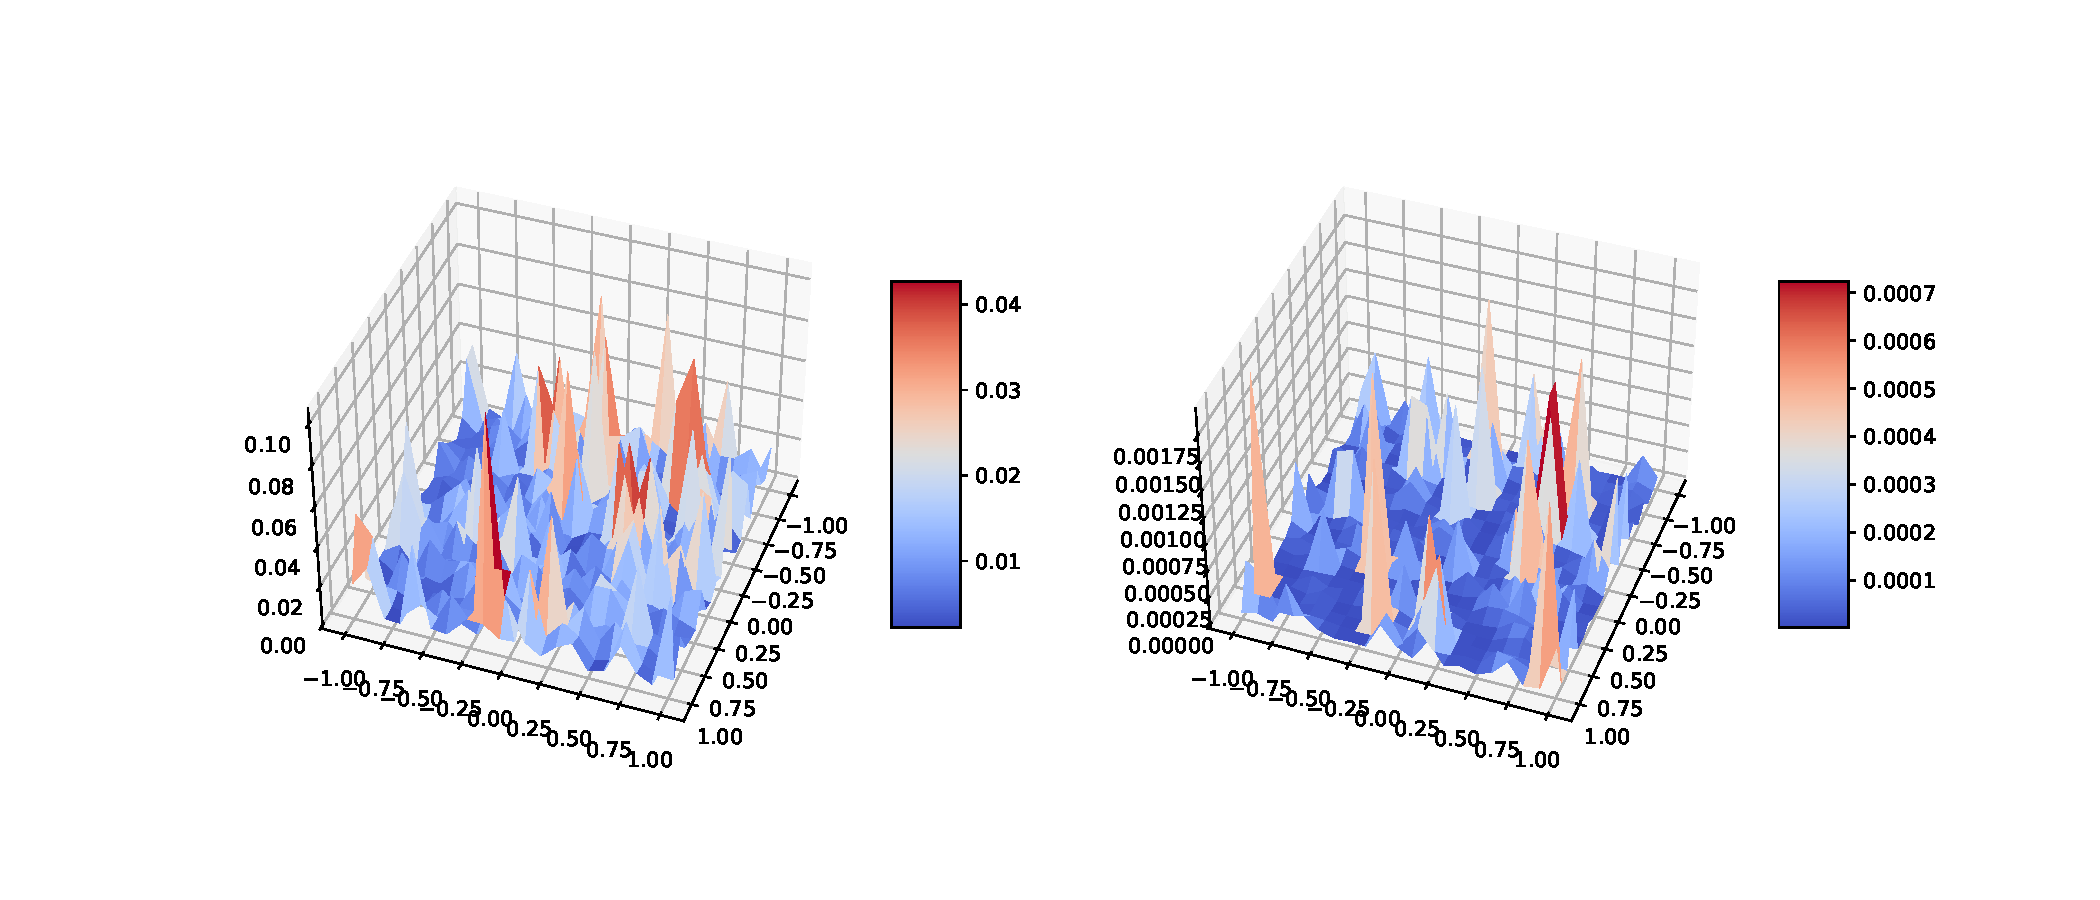
\includegraphics[width=0.8\textwidth]{img/loss_random_1_2.pdf}
        \caption*{3D loss surfaces $L_k$ and $(L_{k+1}-L_k)^2$ for small $k$.}
    \end{figure}
\end{frame}

% Slide 5: Falling Action
\begin{frame}{User Scenario: Falling Action}
    \begin{figure}
        \centering
        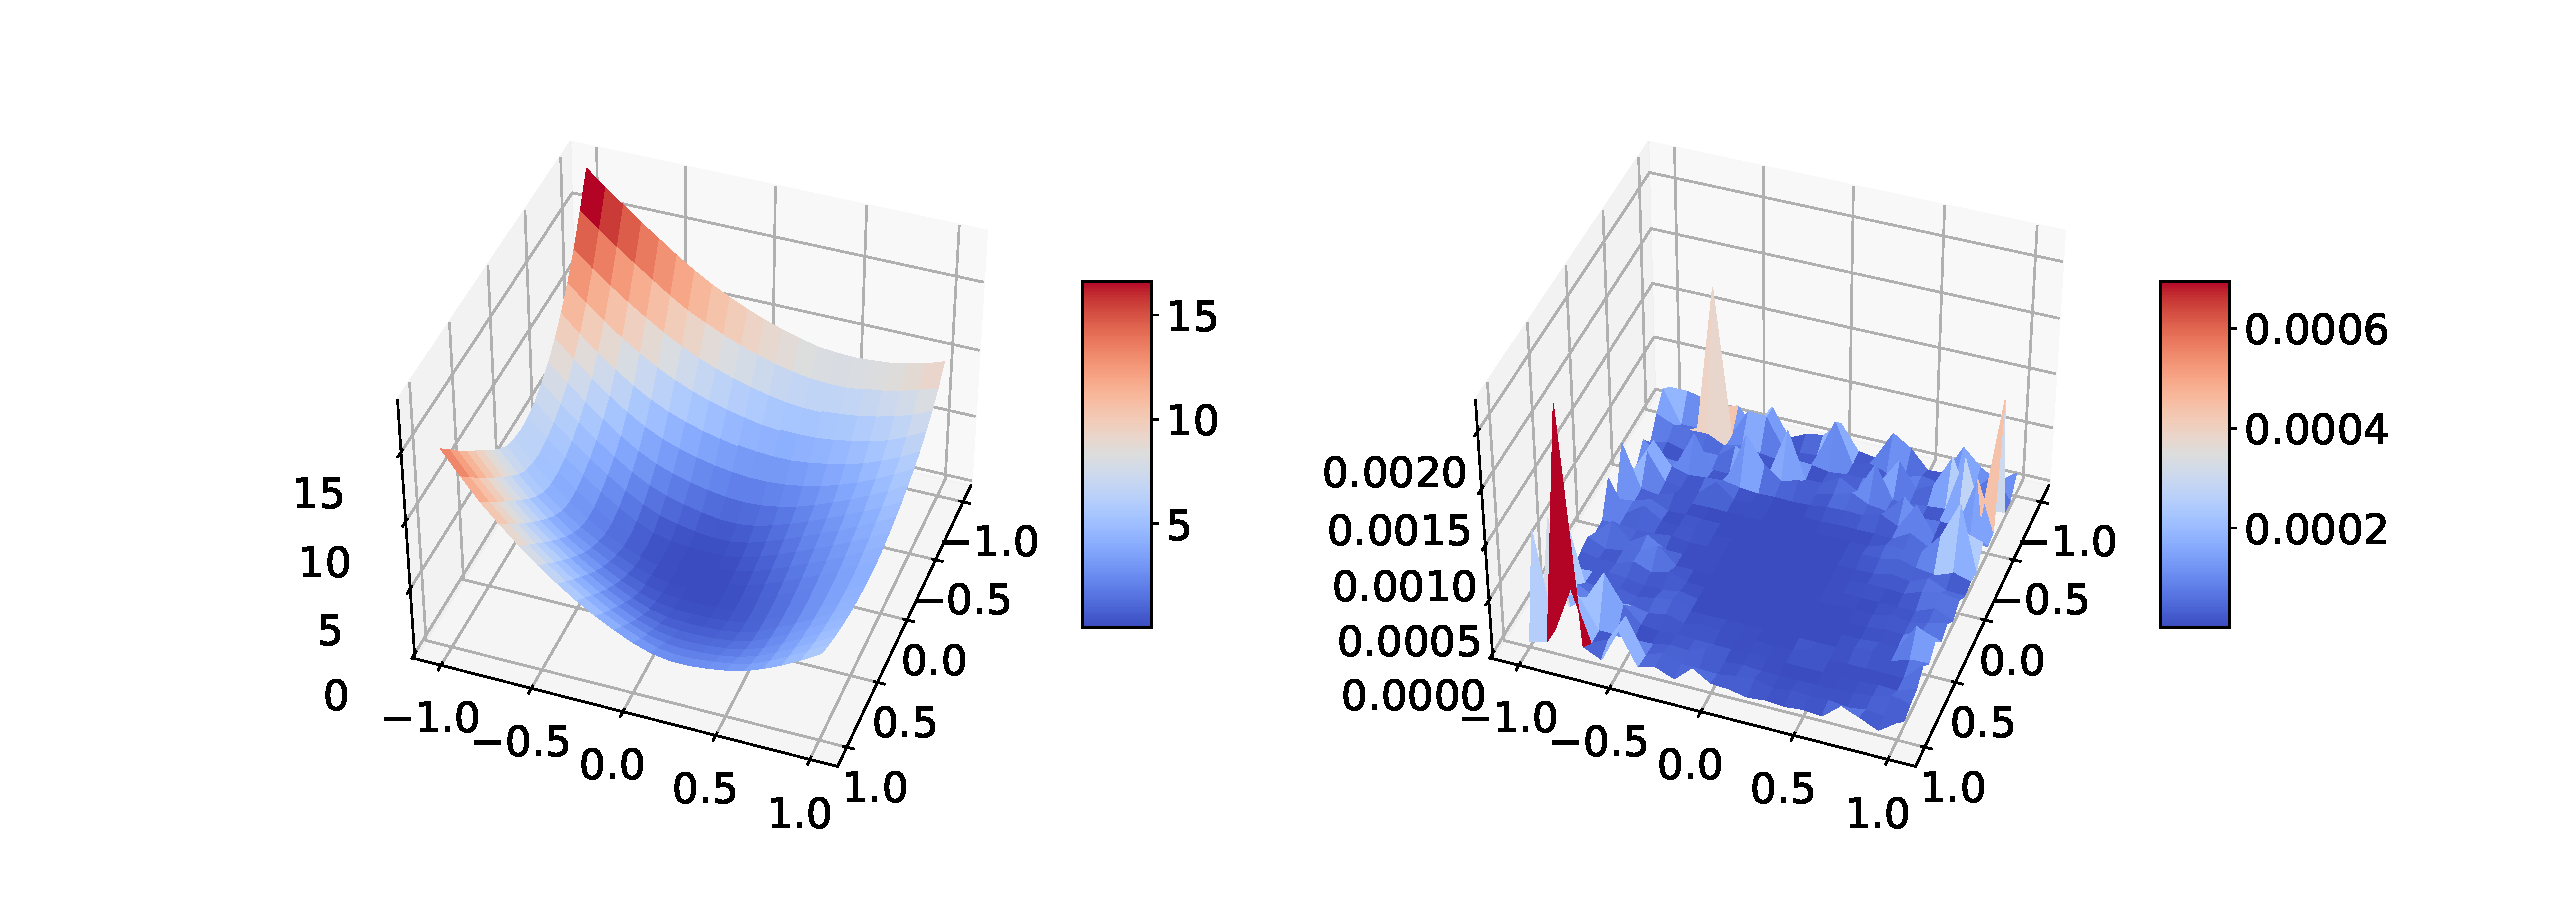
\includegraphics[width=0.8\textwidth]{img/loss_eigen_-2_-1.pdf}
        \caption*{3D loss surfaces $L_k$ and $(L_{k+1}-L_k)^2$ for large $k$.}
    \end{figure}
\end{frame}

% Slide 6: Resolution
\begin{frame}{User Scenario: Resolution}
    \begin{figure}
        \centering
        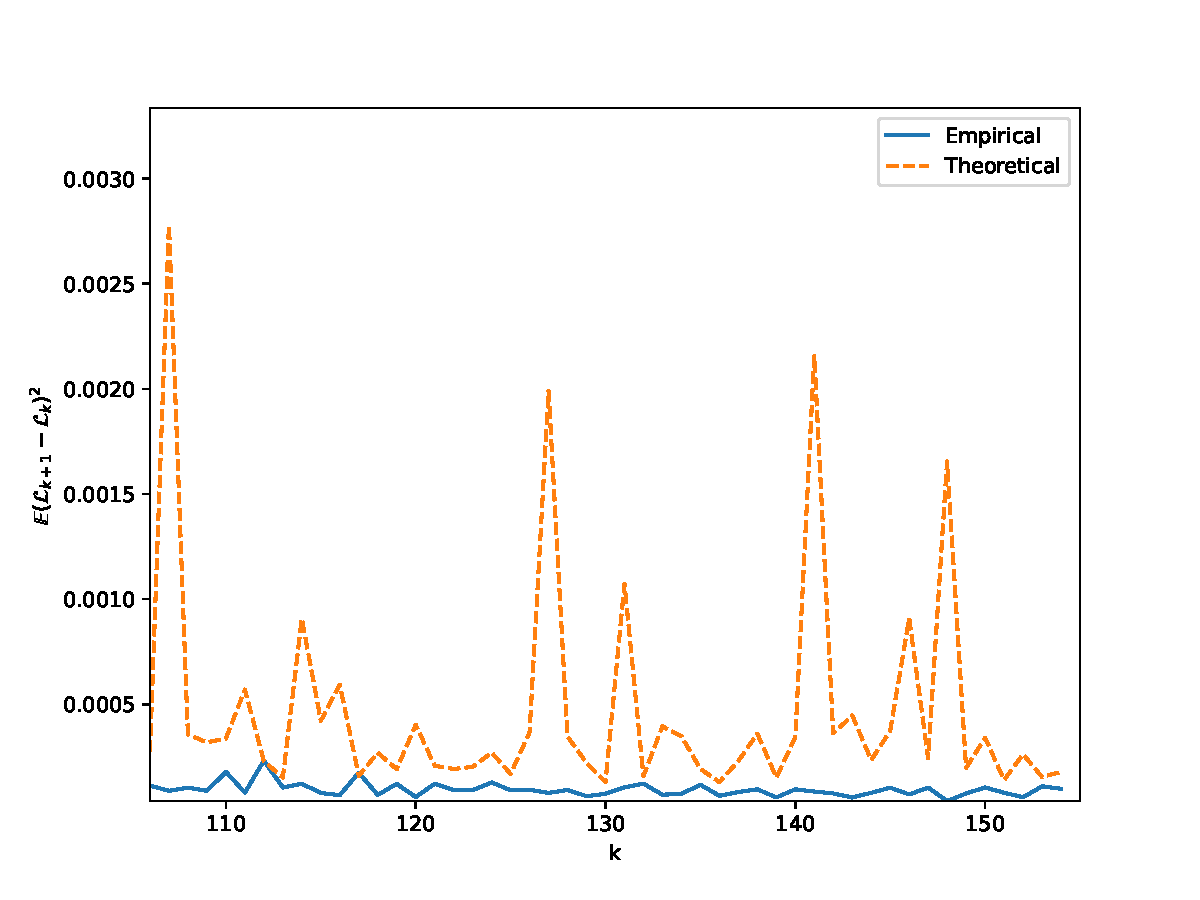
\includegraphics[width=0.7\textwidth]{img/delta_border_1_10_64.pdf}
        \caption*{Decay of $\Delta_k$ and $\Delta_k\cdot k^2$.}
    \end{figure}
\end{frame}

% Slide 7: Prototype – Methodology
\begin{frame}{Prototype: Methodology}
    \begin{itemize}
        \item Compute top $d$ eigenvectors of Hessian $H(w^*)$ via iterative power method.
        \item Form low-dimensional coordinate $\theta$ such that $w = w^* + P\theta$, $P=[e_1,\dots,e_d]$.
        \item Estimate $\Delta_k=E[(L_{k+1}-L_k)^2]$ via Monte Carlo in this subspace.
    \end{itemize}
\end{frame}

% Slide 8: Prototype – Formula
\begin{frame}{Prototype: Theoretical Estimate}
    \vspace{1em}
    \centering
    $\displaystyle
        \Delta_k\approx\frac{\sigma^4}{4}\Biggl(2\sum_{i=1}^d(\lambda_i^{(k+1)}-\lambda_i^{(k)})^2+\bigl(\sum_{i=1}^d(\lambda_i^{(k+1)}-\lambda_i^{(k)})\bigr)^2\Biggr)$
    \vspace{1em}
\end{frame}

\end{document}
